\chapter{基于图过滤的程序依赖图表征学习}
\label{chap:PDG}
本章主要对本文提出的基于图过滤的程序依赖图表征学习方法进行详细介绍,首先介绍其基本思想,其次阐述其具体方法设计与实现,最后进行实验验证。
\section{研究动机}
本文针对现有存在的问题,

程序依赖图PDG是程序的一种图形表示,所含结构信息最多,能够表示程序的控制依赖,数据依赖以及地址依赖等关系,是一种带有标记的有向多重图。程序依赖图PDG结点代表语句,边代表依赖关系,依赖关系包括数据依赖和控制依赖。通过将程序表示为图的形式使得模型能够更好地理解代码中不同部分之间的依赖关系。现有的方法大多通过图匹配的方法,将PDG图中的控制流和数据流编码为一个紧凑的语义特征矩阵,其中每个元素都是一个高维的稀疏二值特征向量,通过寻找矩阵之间的相似模式来判定克隆代码。但这些方法通常需要消耗大量的时间和空间,计算开销大。
\section{PDG表征方法方法设计}
本节将介绍基于图过滤的程序依赖图表征学习方法设计与实现, 

\subsection{框架概述}
基于图过滤的程序依赖图表征学习:

\subsection{图过滤机制}
针对上述问题,本课题引入过滤机制,通过收集PDG的简单特征来过滤掉明显不可能为克隆的PDG对。具体的,根据PDG的节点个数、控制边数、执行边数、数据边数、声明节点数、函数调用数、传入参数、传出参数等代表特征进行过滤,在大幅减少候选PDG对规模的同时,保证真正的克隆对不会被过滤掉而导致整体克隆检出率的降低。

\subsection{程序依赖图表征学习}
对于提取到的程序依赖图,本课题拟通过图卷积神经网络将其转换成向量。图卷积神经网络是一种特殊的前馈神经网络结构,为减少网络中参数个数,用卷积层来代替传统的全连接层,提高神经网络的训练效率,卷积神经网络可以提取信息最多的数据特征,生成一个固定大小的向量表示结构,从而挖掘深层次的语法和语义信息,在代码克隆检测任务中有较好的性能表现。


\section{PDG表征方法具体实现}
\label{sec:achieve}
在介绍具体实现之前,本节首先给出PDG表征方法的输入:经过\ref{subsec:Preprocess}小节的代码预处理阶段,得到示例代码片段\ref{fig:code}中$C_{a},C_{b}$对应的程旭依赖图,如图\ref{fig:pdgcode}所示。
\begin{figure}[htbp]
  \centering  %居中
  \subfigure[C语言代码片段$C_{a}$对应的PDG]{   %第一张子图
      \centering    %子图居中
      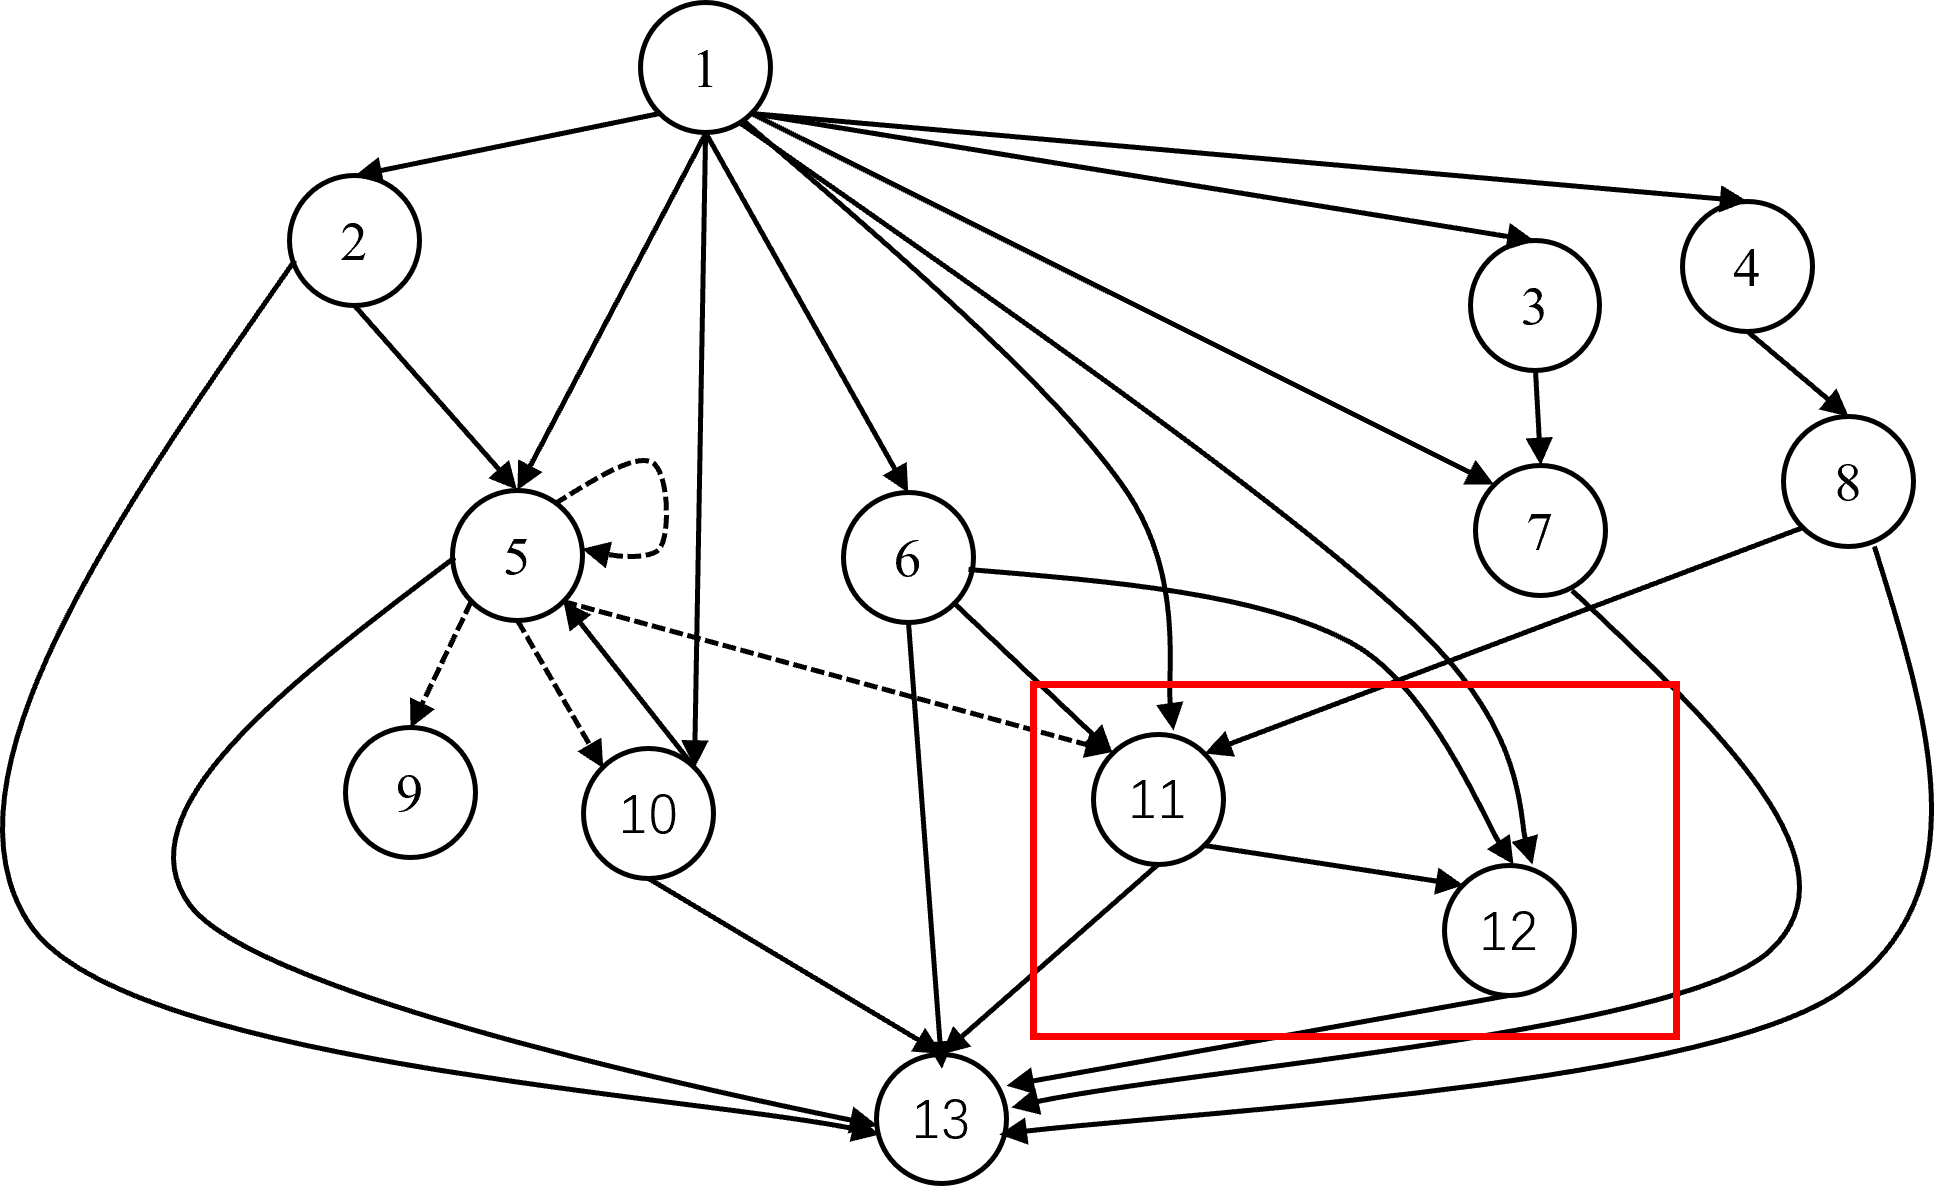
\includegraphics[width=0.85\textwidth]{figures/pdg1}  
      \label{fig:pdg1} %引用标签
  }
  \qquad
	%让图片换行,
  \subfigure[C语言代码片段$C_{b}$对应的PDG]{ %第二张子图
      \centering    %子图居中
      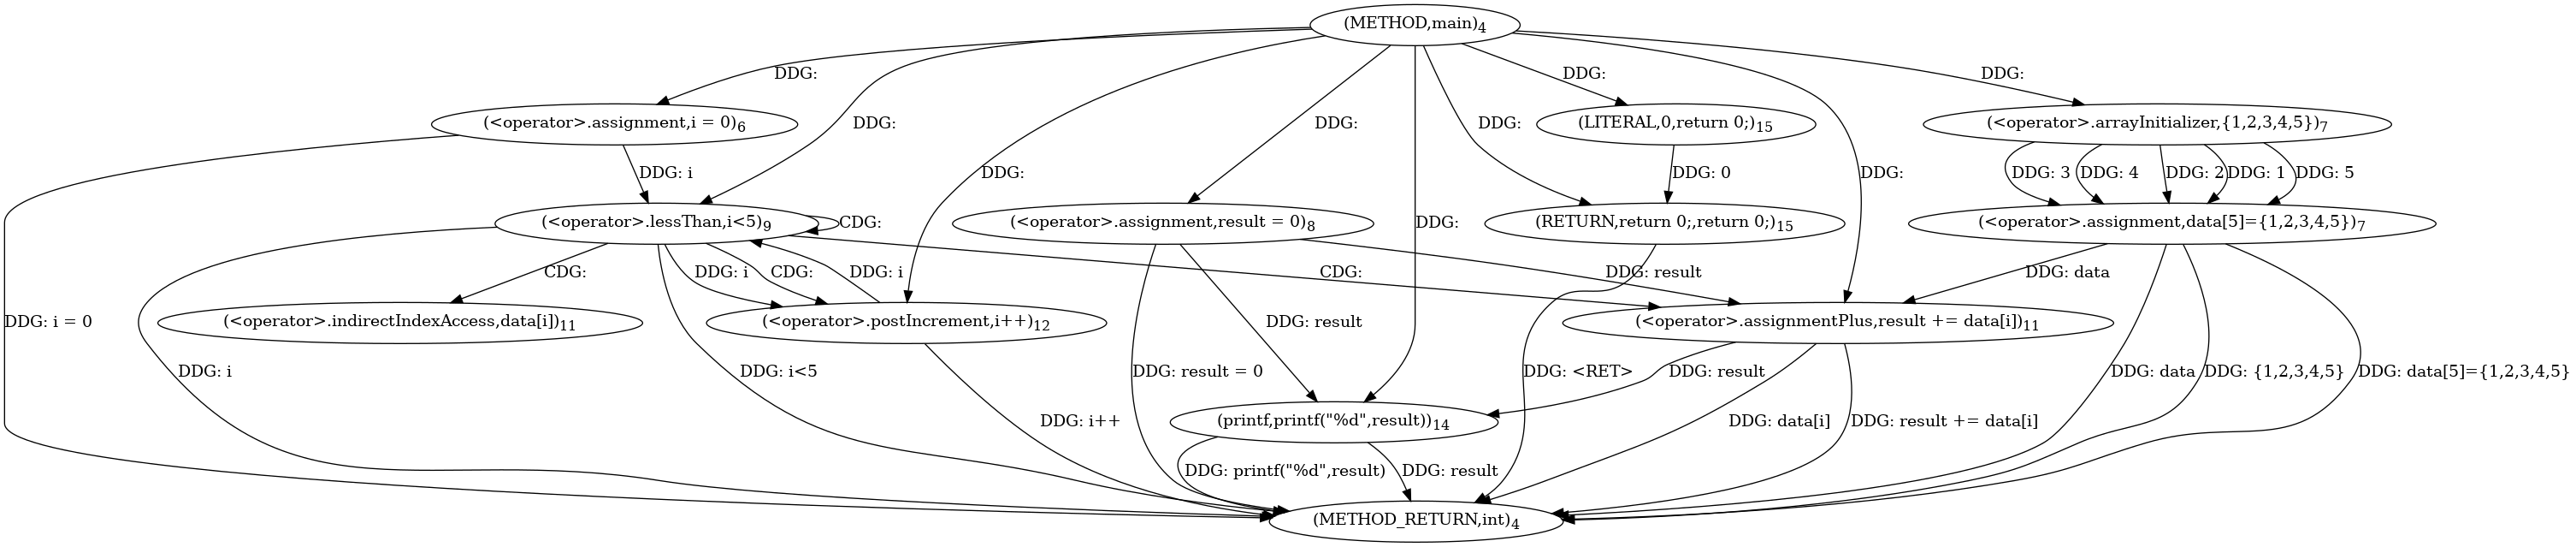
\includegraphics[width=0.85\textwidth]{figures/pdg2}
      \label{fig:pdg2} %引用标签
  }
  \caption{示例源代码对应的程序依赖图}    %大图名称
  \label{fig:pdgcode}    %图片引用标记
\end{figure}


\section{实验验证}
为了验证基于图过滤的程序依赖图表征学习方法的有效性,本文
\subsection{实验设计}
和3.3.1 相同
\subsection{图过滤机制消融实验结果}
消融对比实验:体现图过滤机制的有效性

基于PDG的GCN

基于PDG的+图过滤的GCN


\begin{table}
  \centering
  \caption{图过滤机制实验结果} %{tab:category}
  \begin{tabular*}{0.9\textwidth}{@{\extracolsep{\fill}}cccc}
  \toprule
    对比			&P		&R		&F1 \\
  \midrule
    基于PDG的GCN			&0.xx	&0.xx		&0.xx \\
    基于PDG的+图过滤的GCN			&0.xx		&0.xx		&0.xx \\
  \bottomrule
  \end{tabular*}
\end{table}

\section{本章小结}
本章



